\chapter{Einführung in das Projekt}
Im diesem Kapitel werden verwendete Technologien erläutert. Dabei wird auf die Eigenheiten der Verbindung zur Drohne und den Sensoren eingegangen.

\section{Verwendete Technologien}
Im Projekt kommen 3 Schnittstellen und ein Software-Protokoll zum Einsatz. Sie werden in dieser Reihenfolge erläutert.
\subsection{Wireless Local Area Network}
\gls{wlan} wird als Oberbegriff für lokale Funknetzwerke der IEEE 802.11 verwendet. Es ermöglicht eine drahtlose Datenübertragung und -verarbeitung. Die Geräte senden im 2,4 GHz (ISM-Band) oder 5 GHz Frequenzband. Meist wird es genutzt um mobilen Endgeräten einen Netzzugang zum Internet bereitzustellen. Andererseits kann auch die Reichweite eines kabelgebundenen Netzwerks durch das Überbrücken an schwer zugänglichen Stellen erweitert werden.
%WLAN-Fähigkeit in Endgeräten durch Funkmodul: WLAN-Adapter (= Schnittstellenkarte in Erweiterungssteckplatz auf der Hauptplatine)

Bei der Verwendung von \gls{wlan} ergeben sich folgende Einschränkungen:
\begin{itemize}
    \item Geringe Reichweite (ca. $20$-$30m$)
    \item Schwankende Datenrate, Störanfälligkeit, unzuverlässige Verbindung
    \item Teilung der verfügbaren Bandbreite über alle Teilnehmer
    \item Langsamer als vergleichbare kabelgebundene Techniken
\end{itemize}

Zum Aufbau eines Netzwerkes muss eine Basisistation als Hotspot (auch \enquote{Wireless Access Point} oder \enquote{Gateway} genannt) eingerichtet werden, mit der sich Clients verbinden können. Daten können nur zwischen Client und Basisistation ausgetauscht werden, nicht aber zwischen Client und Client.

Eine Kommunikation erfolgt durch weitere aufbauende Protokolle. Zwangsläufig kommen die Netzwerkprotokolle IP und TCP/UDP zum Einsatz.

Das IP-Protokoll benennt Addressen im Netzwerk. Die Basisistation muss alle beteiligten Geräte und deren Addressen vermerken und ist meist auch für die Verteilung der Adressen zuständig (DHCP-Server Funktion zum Zuweisen der Addressen).

Mit dem TCP-Protokoll wird Vermittlung und Transport von Datenpaketen sichergestellt:
\begin{itemize}
    \item Protokolle bestimmen Ablauf der Kommunikation zwischen den Systemen %(Sammlung von Regeln zum Aufbau, Austausch, Ende)
    \item Sorgt dafür, dass Datenpakete innerhalb eines dezentralen Netzwerks beim Empfänger ankommen
	\item Verbindungsorientiert, Verhindert von Datenverlust
    \item Aufteilung von Dateien und Datenströmen
    \item Datenpakete den Anwendungen zuordnen
	\item Virtuelle Ende-zu-Ende-Kommunikation (Sender und Empfänger während Verbindung dauerhaft in Kontakt)
\end{itemize}
Es treten weitere Verfänglichkeiten auf:
\begin{itemize}
    \item Empfänger bestätigt jedes empfangene Datenpaket
    \item Keine Bestätigung führt zu Wiederholung Sendevorgang
	\item Verbindungaufbau über Three-Way-Handshake (Verbindungswunsch vom Client, Bestätigung Anfrage durch Server, Verbindungswunsch durch Server, Bestätigung Client)
\end{itemize}

Somit ist die Übertragung über TCP besonders langsam. Im Außenbereich bei größeren Entfernung kann es zu Verbindungsabbrüchen kommen.

Im Gegensatz dazu arbeitet das UDP-Protokoll nach dem Fire-and-Forget-Prinzip. Daten werden ohne Kontrolle gesendet. Es kommt beim bspw. beim Streaming von Bild- und Ton Inhalten zum Einsatz. Beim Datenverkehrt über \gls{wlan} wird stark von UDP abgeraten, denn auftretende Verluste können nicht korrigiert werden.

\subsection{Serielle Schnittstelle}
Die Serielle Schnittstelle wird in der Fachwelt als \gls{uart} bezeichnet.

Sie verbindet 2 Kommunikationspartner und besteht aus 1 bzw. 2 Leitungen. Letzterer Fall kommt im Projekt für eine bidirektionale Kommunikation zum Einsatz: je eine Leitung wird für die Verbindung in eine Richtung verwendet. Die Leitungen heißen respektive Transmit (Tx) und Receive (Rx). Sie werden jeweils über Kreuz mit den Endstellen verbunden, sodass zwei Tx-Rx Paarungen entstehen. Zusätzliche Leitungen können für die Synchronisation (bspw. Aktivschalten des Kanals) vorkommen.

Für die Kommunikation müssen beide Teilnehmer in den Parametern übereinstimmen:
\begin{itemize}
    \item Baudrate (Übertragungsgeschwindigkeit je Zeichen)
    \item Wortlänge (Bit je Übertragung)
    \item Parity Bit (optional am Ende jeden Wortes)
    \item Länge des Stopbits (Zeitdauer in Baud)
\end{itemize}

Je nach Anwendungszweck ist \gls{uart} auf eine bestimmte Leiterspannung ausgelegt. Bei der Verwendung von Microcontrollern kommt häufig ein Pegel von $3.3V$ oder $5V$ zum Einsatz. Im Leerlauf weisen die Leitungen ein High (hoher Pegel) auf. Zu Beginn einer Übertragung wird das Startbit auf Low gesetzt. Es folgt eine Wortlänge and Datenbits, ein Parity Bit und ein Stopbit.\newline

Sind alle Parameter gleich können ohne weitere Absprache digitale Werte versendet/empfangen werden. Die intterpretation erfolgt dann von entsprechender Software.

\subsection{Inter-Integrated Circuit}
Mit \gls{i2c} können Microcontroller und Peripherie beliebig verbunden werden. Das System erlaubt das Zusammenschalten von einem Master mit bis zu 127 Slaves.

Es können Geräte unterschiedlicher Spannungspegel verbunden werden. Die Leitung wird mit dem Minimum der höchsten verträglichen Spannungen der Busteilnehmer betrieben. Alle Teilnehmer müssen diese als High interpretieren.

\gls{i2c} verwendet 2 Leitungen, genannt Data (SDA) und Clock (SCL). Auf der Leitung Clock wird vom Master ein Takt erzeugt. Dieser kann aber auch von einem Slave auf Low (niedriger Pegel) gehalten (Verbindung gegen Masse) werden, wenn dieser noch Rechenzeit zur Verarbeitung benötigt, fachsprachl. Clock Stretching. Nutzdaten werden bei steigender Flanke der Clock auf der Data Leitung übertragen.

Eine Kommunikation läuft folgendermaßen ab:
\begin{enumerate}
    \item Kommunikationsbeginn durch heruntersetzen der SDA-Leitung während SCL auf High ist
    \item Master schreibt 7 Bit als Adresse des Slave
    \item Master schreibt 8. Bit als Lese- oder Schreib-Bit
    \item Bestätigung durch Slave (Bit auf Low)
    \item Master oder Slave schreibt vorgegebene Anzahl Nutzdaten
    \item (Direktes Fortsetzten der Kommunikation bspw. als Antwort auf Anfrage) 
\end{enumerate}

\subsection{MAVLink}
\gls{mav} ist ein Übertragungsprotokoll welches von der Dronecode Stiftung entwickelt wird\footnote{\url{https://mavlink.io/en/}}. Es wird zur Kommunikation von Drohnen mit derer Peripherie eingesetzt.

Dabei ist \gls{mav} zuständig für das binäre Kodieren von Informationen. Das Protokoll definiert Nachrichten aus einer Auszeichnungssprache (XML) welche dann kompiliert werden. Je nach Gerät wird ein bestimmter Satz Nachrichten implementiert.

Ein \gls{mav}-Netzwerk kann aus bis zu 255 Geräten und Bodenstationen bestehen, die ähnlich einem LAN-Netzwerk, Nachrichten miteinander austauschen. Dabei legt das Protokoll großen Wert auf geringen Overhad in den einzelnen Nachrichten um bei geringer Bandbreite arbeiten zu können.

Trotzdem implementiert \gls{mav} Mechanismen zur Überwachung der Datenkonsistenz. Zum Einsatz kommen Paketnummern und CRC-Checksummen. Somit kann es Fehler/Störungen in der Übertragung erkennen und ausgleichen. Es ist für eine Übertragung über verschiedene, auch einfache, Kommunikationskanäle (bspw. RC-Funktempfänger) geeignet.

\section{Beschreibung der Drohne}
Eine Drohne steht seit den Ausarbeitungen \cite{wirthErweiterungBestehendenDrohne2022} und \cite{wirthErweiterungBestehendenDrohne2022a} bereit. Im Rahmen des Projektes \cite{markusreinErweiterungBestehenderDrohnen2023} wurden die Ultraschallsensoren neu befestigt. Ein Gesamteindruck der Drohne ist gegeben in den Bildern \ref{fig:drohne_schraeg_vorn} und \ref{fig:drohne_oben}. Nach einem bereits älteren Unfall wurde die Halterung des linken Standfußes per 3D-Druck erneuert, siehe Bild \ref{fig:drohne_fuss}. Das Modell des Bauteils stammt von \footnote{\url{https://www.thingiverse.com/thing:3761929}}. 

\begin{figure}[h]
    \centering
    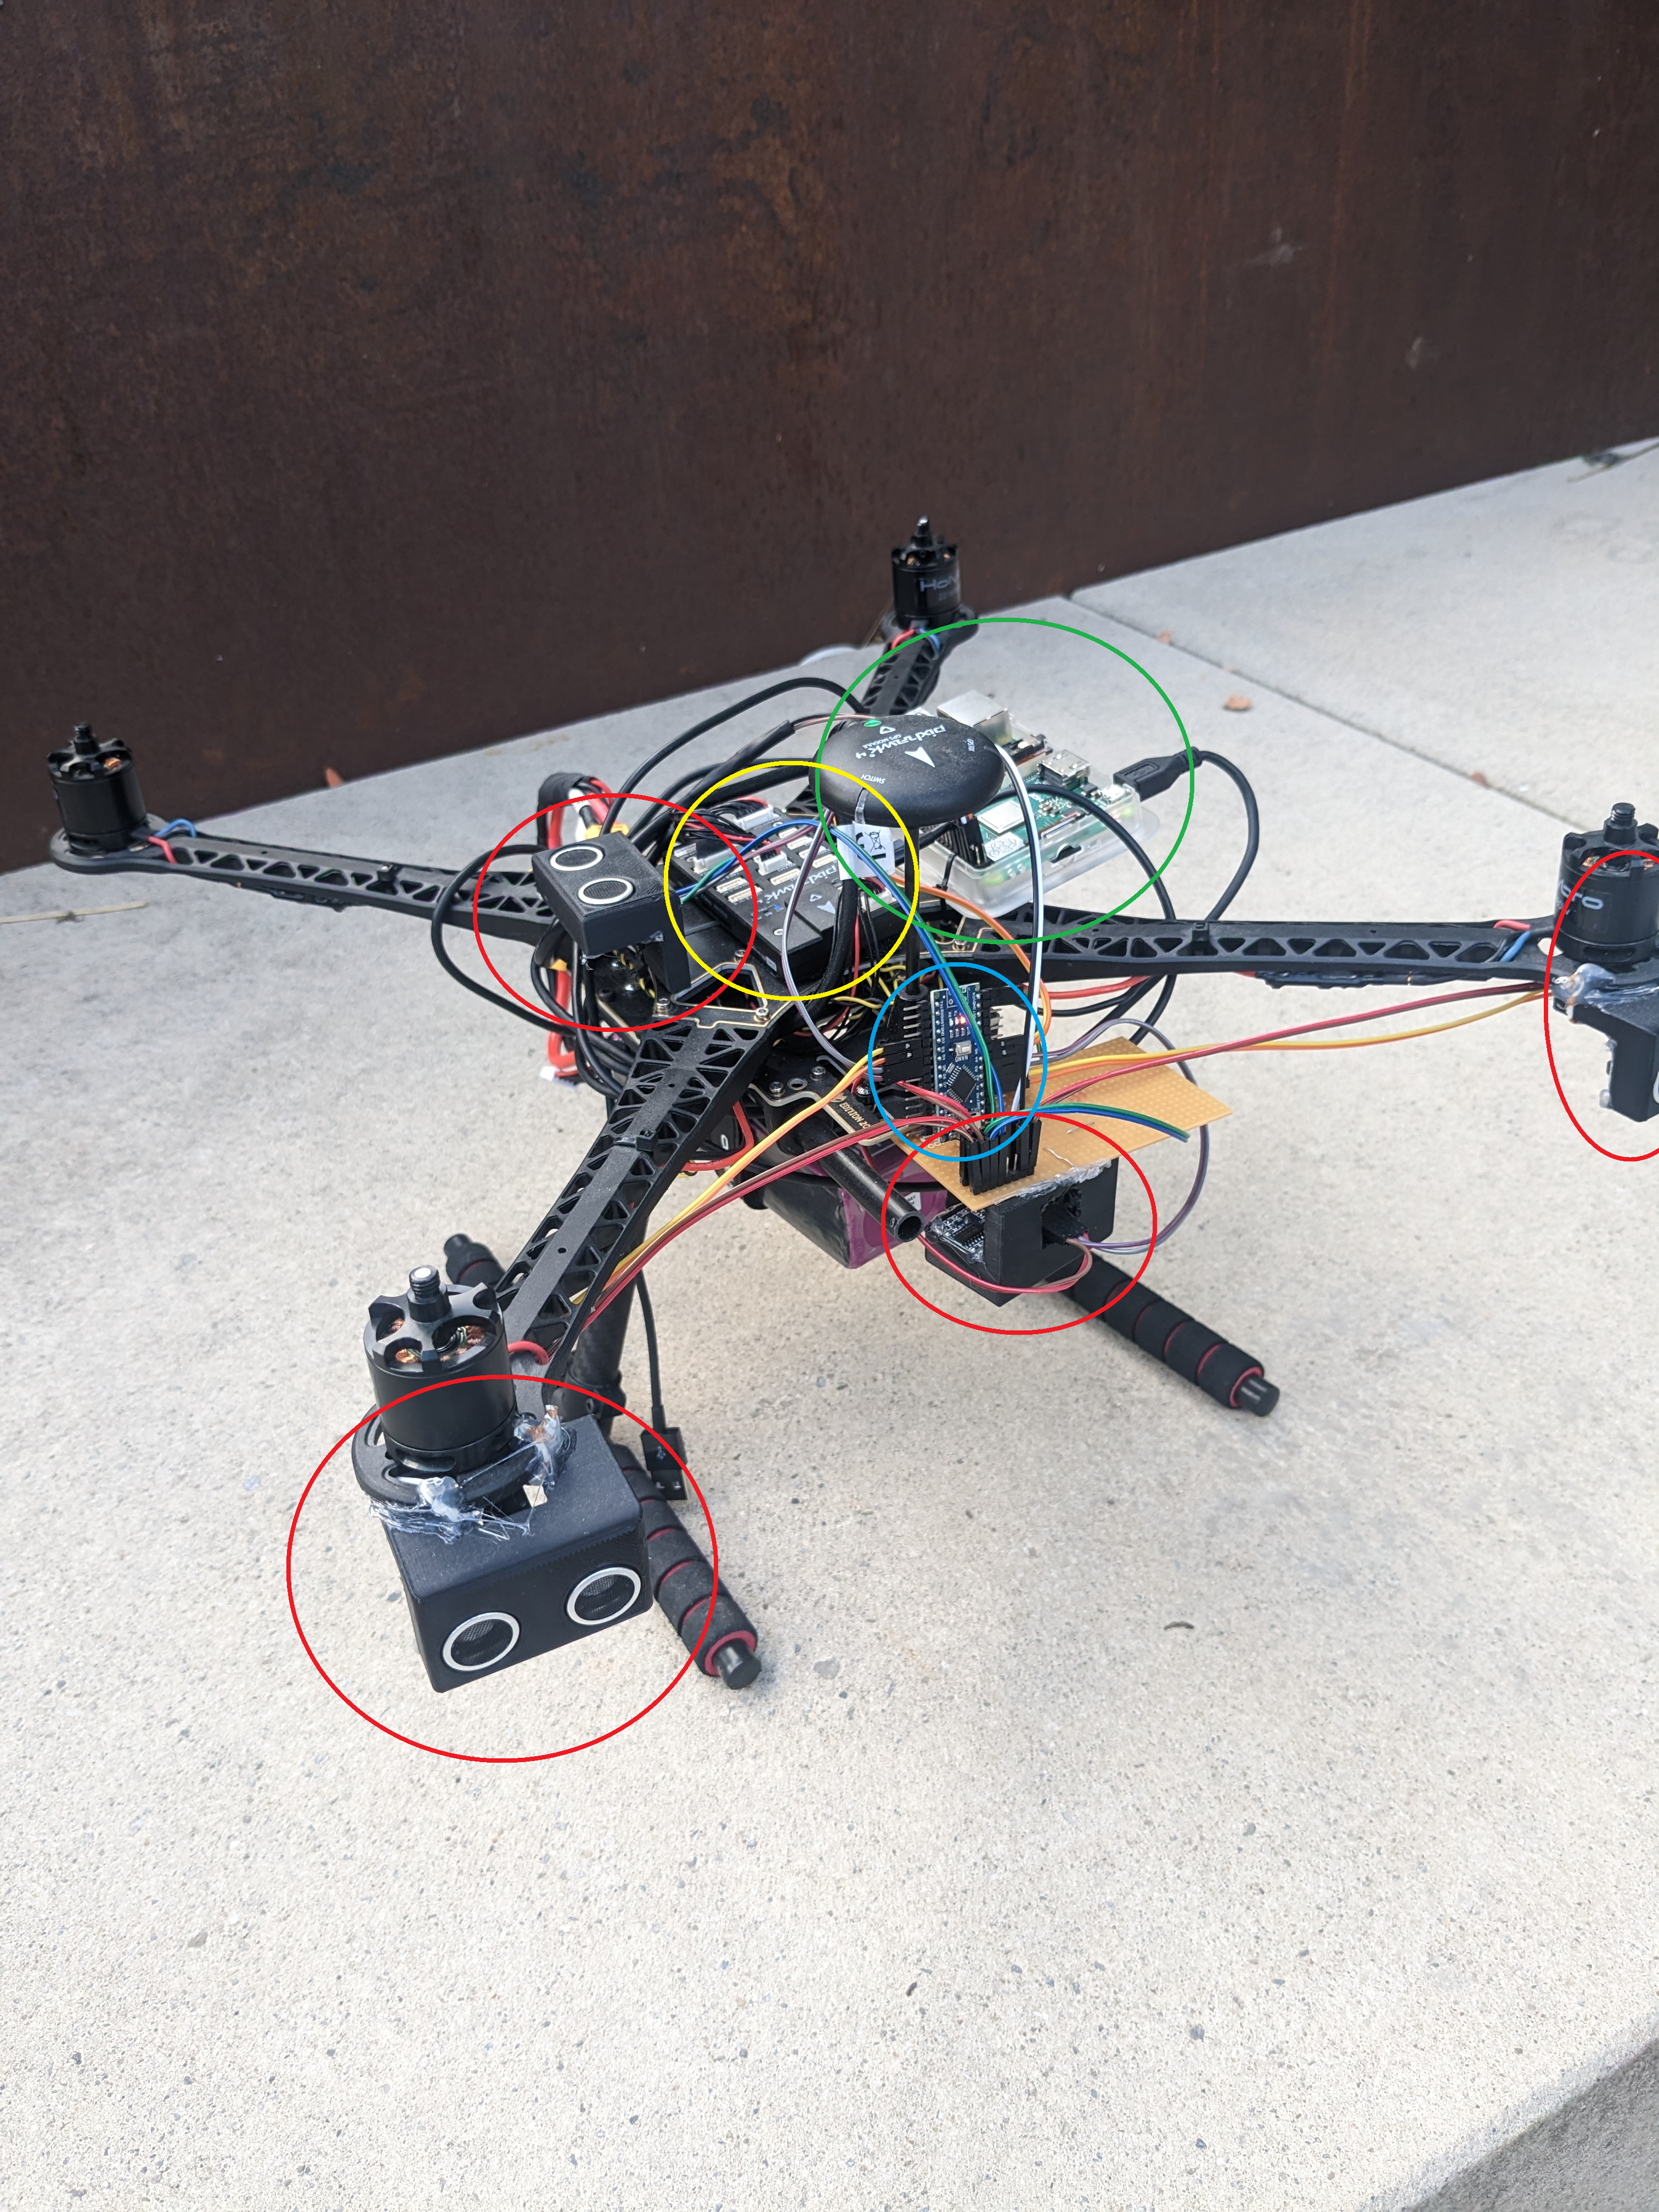
\includegraphics[width=0.8\textwidth]{images/drohne_schraeg_vorn.png}
    \caption[Gesamtansicht Drohne vorn]{Gesamtansicht Drohne vorn: viermal rot umrahmt die Ultraschallsensoren, blau umrahmt der Arduino (Auslesen der Sensoren), grün umrahmt der Raspberry Pi (Bordcomputer), gelb umrahmt der Flugcontroller (\acrshort{px4})}
    \label{fig:drohne_schraeg_vorn}
\end{figure}

\begin{figure}[h]
    \centering
    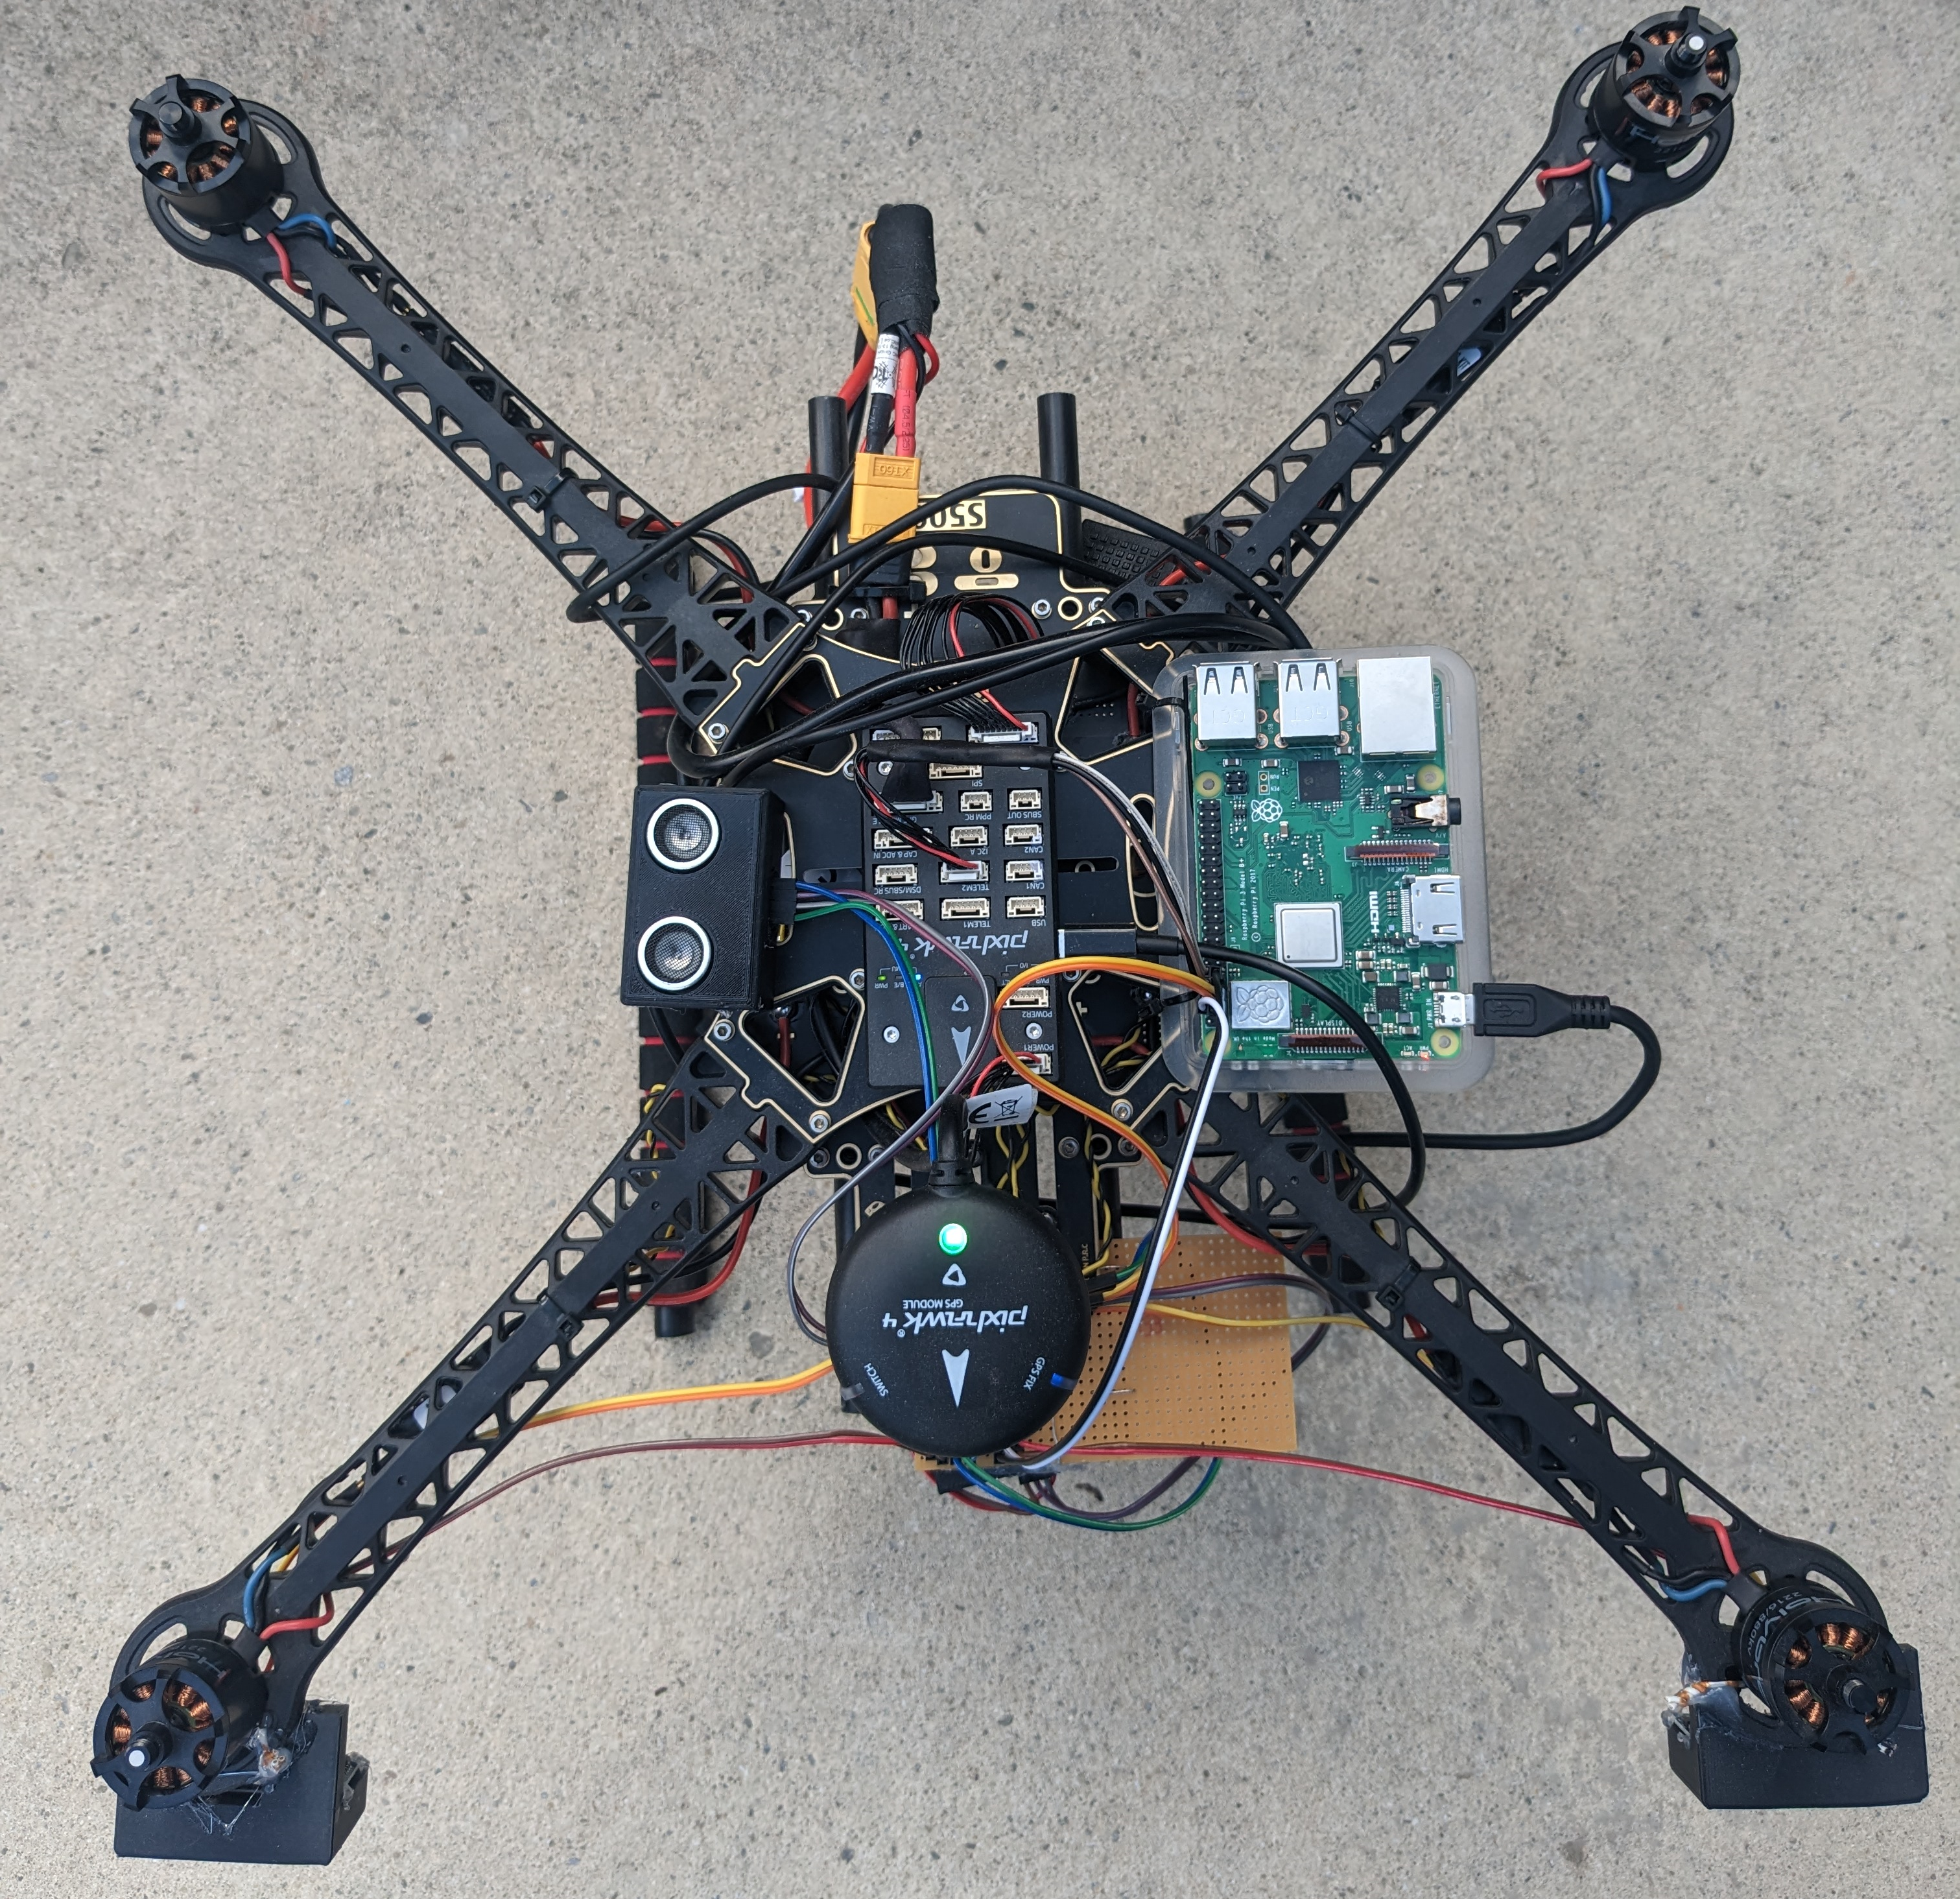
\includegraphics[width=0.8\textwidth]{images/drohne_oben.png}
    \caption[Gesamtansicht Drohne oben]{Gesamtansicht Drohne oben}
    \label{fig:drohne_oben}
\end{figure}


\begin{figure}[h]
    \centering
    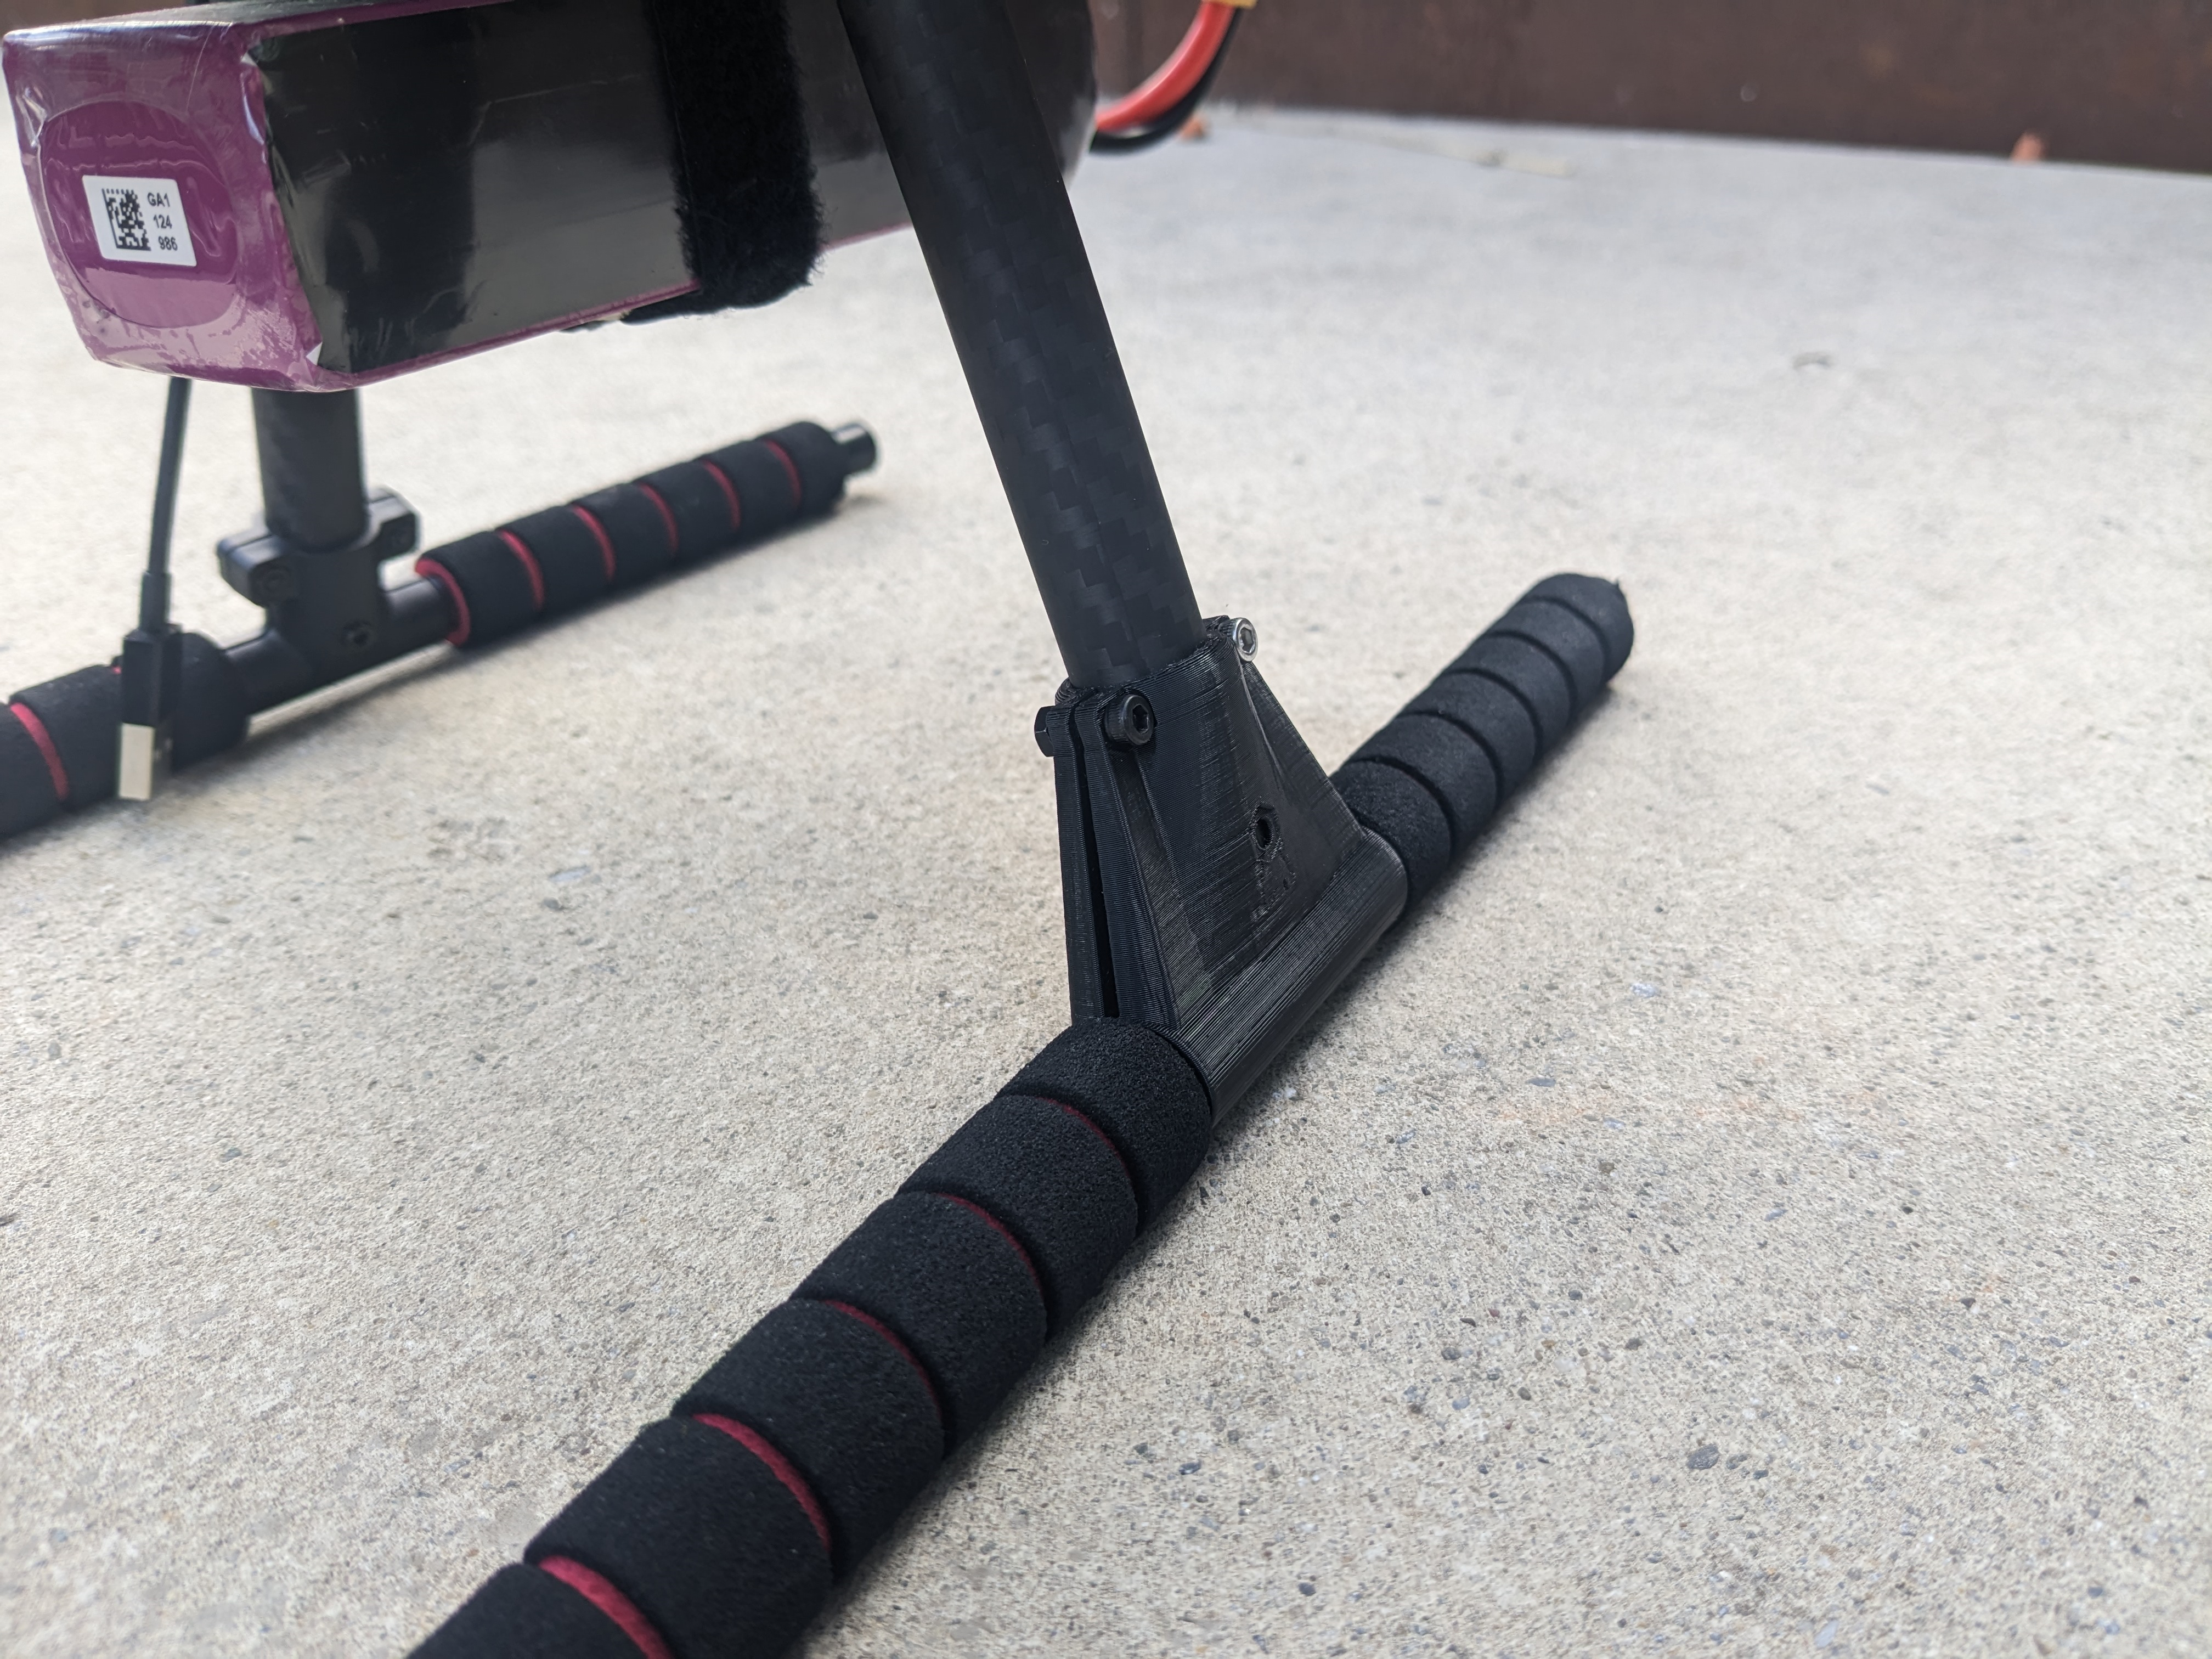
\includegraphics[width=0.8\textwidth]{images/drohne_fuss.png}
    \caption[Standbeine der Drohne]{Standbeine der Drohne: das T-Stück zur Verbindung des Linken Beines mit dem Fuß wurde ausgewechselt}
    \label{fig:drohne_fuss}
\end{figure}

% Die Drohne kann mit Methoden der Regelungstechnik als adaptives System beschrieben werden. Dabei dient der Flugcontroller als Regler, die Motoren als Steuerstrecke, und Bordcomputer sowie Bodenstation zur Identifikation und Modifikation der Parameter.
Die Drohne in ihrer Ausgangslage, ohne automone Flugfähigkeiten, kann durch 3 wesentliche Bestandteile beschrieben werden. Diese sind aufgelistet in Tabelle \ref{tab:system_intro}.
Nähere Beschreibungen folgen in den nächsten Kapiteln zusammen mit der Erläuterung zu den angebauten Ultraschallsensoren. Zusammen bilden sie ein System wie in Bild \ref{fig:system_intro} gezeigt. Im Flugbetrieb werden von der Bodenstation Flugbefehle (feste Zielkoordinaten, relative Koordinaten, oder manuelle Motoransteuerung) an den Bordcomputer und von diesem weiter an den Flugcontroller, geschickt. Mehr Details zur Steuerung mit der Bodenstation in \cref{chap:intro_capabilities}.

\begin{table}[!ht]
    \caption{Systemübersicht Drohne und Bodenstation}
    \begin{tabularx}{\textwidth}{l | X | X | X }
    & \multicolumn{2}{c |}{Drohne} & \\
    & Flugcontroller & Bordcomputer & Bodenstation \\ \hline
    Funktion & Autopilot-Software liest Sensoren und steuert Motoren der Drohne & Bereitstellung \acrshort{wlan}-Netzwerk zur Verbindung von Autopilot und Bodenstation & Parametrierung und Steuerung der Drohne\hfill \\ \hline
    Hardware & Pixhawk 4 & Raspberry Pi 3B+ & PC und/oder Smartphone \hfill \\ \hline
    Software & PX4 & MAVLink-Router% \newline -ROS-Umgebung \newline -Avoidance \newline Hindernisse, Trajektorie, Flugcontroller bedienen, Ultraschallsensoren
    & QGroundControl \hfill \\
    \label{tab:system_intro}
    \end{tabularx}
\end{table}

\subsection{Flugcontroller}
Der Flugcontroller vom Typ \gls{px4} ist Bestandteil der ursrpünglichen Drohne. Er allein verfügt über die Steuerung der Drohne, kann aber Kommandos von anderer Peripherie erhalten.

Er verfügt sowohl über integrierte Sensoren: Beschleunigungssensor, Kompass und Barometer; als auch dass er mit der \acrshort{gps}-Antenne verbunden ist. Weiterhin besitzt er Anschlüsse zu den \gls{esc} der Motoren. Außerdem kann an ihm eine RC-Fernsteuerung angeschlossen werden, allerdings wird für dieses Projektes keine Fernsteuerung benötigt.
Weitere Sensoren oder Aktoren lassen sich über verschiedene Schnittstellen an den Flugcontroller anschließen. Für den Betrieb ist der Bordcomputer per \acrshort{uart}-Verbindung angeschlossen.\newline

Die Software des Flugcontrollers wird PX4-Flightstack genannt. Mit ihr lassen sich verschiedene Microcontroller, embedded Systems, oder PCs zum Steuern von Robotern, Fahrzeugen oder Drohnen ausgestatten. Sie wird von der Dronecode Stiftung\footnote{\url{https://www.dronecode.org/}} herausgegeben.

\subsection{Bordcomputer}
In der Ausarbeitung \cite{markusreinErweiterungBestehenderDrohnen2023} wurde ein \acrlong{rpi} Model 3 B+ an der Drohne montiert.

Die Speicherkarte mit Betriebssystem und Software kann aus dem vorherigen Projekt übernommen werden. Installiert ist das 32-Bit Betriebssystem Raspberry Pi OS und das Programm \enquote{mavlink-routerd} mit dem \acrshort{mav}-Packete zwischen mehreren Schnittstellen weitergeleitet werden können. Letzteres startet automatisch beim Hochfahren des Systems und verbindet sich mit dem Flugcontroller (falls dieser eine Stromversorgung hat).

Die Schnittstellen des \gls{rpi} sind folgendermaßen konfiguriert:
\begin{itemize}
    \item \gls{uart} für Verbindung mit Flugcontroller
    \item \gls{i2c} für Verbindung mit Arduino
    \item \gls{wlan} eingerichtet als Hotspot
\end{itemize}

\subsection{Bodenstation}
Sie dient der Instrumentation der Drohne. 

Als Bodenstation stehen verschiedene Programme sowohl für Computer als auch Smartphone zur Verfügung\cite{ardupilotdevteamChoosingGroundStation}:
\begin{itemize}
    \item Mission Planner
    \item APM Planner 2.0
    \item QGroundControl
    \item DroidPlanner 3
    \item AndroPilot
\end{itemize}
Im Projekt eingesetzt wird \textit{QGroundControl}, denn es ist das Programm der Dronecode Stiftung, verfügt also über die beste Unterstützung.\newline

QGroundControl baut automatisch eine Verbindung mit dem Flugcontroller auf, wenn dieser per Kabel mit dem Computer verunden ist, oder der Computer entsprechende UDP-Packete empfängt. Ersterer Modus kann genutzt werden, um die Firmware des Flugcontrollers zu aktualisieren.

Weiterhin unterstützt QGroundControl die Verbindungsarten Netzwerk und Serielle Schnittstelle. Es könnte direkt auf dem Bordcomputer der Drohne betrieben werden. Weiterhin könnte es die Funktion von \textit{mavlink-routerd} übernehmen und somit Packete über das Netzwerk verteilen.

\subsection{Ultraschallsensoren an der Drohne}
Die Ultraschallsensoren erzeugen analoge Messwerte (Zeitdauer), die ausgewertet werden muss (siehe \cite[Kapitel 4.4]{markusreinErweiterungBestehenderDrohnen2023}). Diese Aufgabe übernimmt im Projekt ein Arduino Nano (Microcontroller).\newline

Der Flugcontroller kann mit einer Reihe offiziell unterstützter Abstandssensoren arbeiten\footnote{siehe \url{https://docs.px4.io/main/en/sensor/rangefinders.html}}. Um einen eigenen Sensor zu entwerfen muss ein entsprechender Adapter an den Flugcontroller angeschlossen und das Protokoll \gls{mav} implementiert werden. Im Rahmen dieser Arbeit werden die digitalen Messwerte hingegen vom Bordcomputer abgefragt und verarbeitet.

Dazu kommt das \gls{i2c}-Protokoll zum Einsatz. Der Arduino reagiert als Slave-Gerät mit der Adresse $8$. Nach der Adresse wird jeweils ein \enquote{Register} geschrieben, der Arduino antwortet mit den Werten der Sensoren. Mehr Details in \cref{chap:arduino_sensors}.

%\paragraph*{}
%Erweiterte Funktionalität wird auf dem Entwicklungsrechner in Containern, in Verbindung mit der Simulation, erprobt. Derartige fertige Anwendungen können dann direkt auf dem Bordcomputer eingesetzt werden. Bestandteile der Software sind:
%\paragraph*{}
%\begin{description}
%    \item[\gls{ros}] 
%    \item[\textit{mavros}:] auf gleicher Ebene angesiedelt wie eine Bodenstation, erlaubt Protokollübersetzung zwischen \gls{mav}- und \acrshort{ros}-Nachrichten für \acrshort{ros}-internen Datenaustausch, empfängt Daten der Drohne und sendet neue Anweisungen zur Drohne
%    \item[Tiefenverarbeitung:] arbeitet direk mit Tiefenbildern aus dem Simulator um eine \enquote{Punktwolke der Umgebung} zu generieren
%    \item[\textit{Avoidance}:] setzt neue Zielpunkte für Drohne anhand von Sensordaten der Drohne und Punktwolke von Kamera
%    \item[\textit{AirSim-Wrapper}:] nicht für Endanwendung benötigt, kommuniziert direkt mit dem Simulationsprogramm und stellt Tiefenbild bereit
%\end{description}
%
%